\documentclass{article}
\usepackage{graphicx}
\usepackage{float}
\usepackage{amsmath}
\usepackage{amsfonts}
\usepackage{amssymb}
\usepackage{hyperref}
\usepackage{esint}
\usepackage[utf8]{inputenc}
\usepackage[a4paper, portrait, margin=0.75in]{geometry}
\setlength\parindent{0pt}
\usepackage[italian]{babel}





\hypersetup{
    colorlinks=true,
    linkcolor=black,
    filecolor=magenta,
    urlcolor=blue,
    pdftitle={Tecnologie internet},
    pdfpagemode=FullScreen,
}


\begin{document}
    \author{kanopo}
    \title{Analisi 1}

    \maketitle
    \tableofcontents

    \listoffigures
    \listoftables



    \section{Insiemi e funzioni}
\subsection{Insieme}

\begin{equation*}
    A = \{1,2,3\}
\end{equation*}

\begin{itemize}
    \item $1 \in A$
    \item $4 \notin A$
\end{itemize}

\subsubsection{Caratteristiche}
\begin{enumerate}
    \item appartenenza di un elemento
    \item un elemento compare una sola volta
    \item no ordine di comparizione
\end{enumerate}

A e B sono due insiemi uguali se ogni elemento di B appartiene ad A e ogni elemento di A appartiene a B.


\textbf{Cardinalità}: numero di elementi in un insieme.

\subsection{Operazioni tra insiemi}
\begin{itemize}
    \item Unione
    \item Intersezione
    \item Differenza
\end{itemize}

\subsection{Completamento di un'insieme}
\begin{equation*}
    C_{(A)} = A^C = \{x : x \notin A\}
\end{equation*}

Esempio:

P è l'insieme naturale dei numeri pari? allora il completamento sono tutti i numeri naturali dispari.


\begin{itemize}
    \item $\mathbb{N}$ sono gli interi positivi $\{1,2,3,\dots\}$
    \item $\mathbb{Z}$ sono gli interi $\{-\infty, \dots, -2, -1, 0, 1, 2, \dots, +\infty\}$
    \item $\mathbb{Q}$ sono i razionali $\{\frac{p}{q} : q,p \in \mathbb{Z}\}$
    \item $\Re$ sono i reali
\end{itemize}

\subsection{Funzioni (applicazioni, trasformazioni, mappe)}
\begin{equation*}
    f: x \rightarrow f(x)
\end{equation*}

Dove la $x$ è il dominio e $f(x)$ è il codominio.

La funzione trasforma l'elemento di un'insieme in un'elemento anche di un'altro insieme.

\subsection{Funzione iniettiva}
\textbf{Definizione:}

$f$ è \textbf{iniettiva} se associa a elementi distinti del dominio a elementi distinti del codominio.

\begin{equation*}
    \forall x_1, x_2 \in X : x_1 \neq x_2 \Rightarrow f(x_1) \neq f(x_2)
\end{equation*}

Se invece le due $x$ sono uguali, le loro $f(x)$ saranno uguali.

\subsection{Immagine di una funzione}

\begin{equation*}
    f : X \rightarrow Y
\end{equation*}

L'immagine di $f$ è il sottoinsieme di $Y$ che contiene tutti gli elementi di $Y$ che si possono ottenere partendo da $X$.

\begin{equation*}
    Im f = \{y \in Y \Leftrightarrow \exists x \in X : y=f(x)\}
\end{equation*}

\textbf{Definizione:}

$f$ è \textbf{suriettia} se $Im f = Y$.

\textbf{Definizione:}

$f$ e \textbf{biettiva} se è suriettiva e iniettiva


\section{Dominio di funzione}

\textbf{Logaritmi:}
\begin{equation}
    \ln(AB) = \ln(A)+\ln(B)
\end{equation}

\begin{equation}
    \ln(\frac{A}{B}) = \ln(A)-\ln(B)
\end{equation}

Sostanzialemte il dominio è quella parte di spazio nel piano dove la funzione è verificata(esiste).



\section{Funzioni invertibili}
\textbf{Definizione:}
Sia:
\begin{equation*}
    f:X \rightarrow Y \Rightarrow g:Y\rightarrow X
\end{equation*} 

$g$ è l'inversa di $f$.

\subsection{Monotonia}

Se:
\begin{equation*}
    \forall x_1,x_2 : x_1<x_2
\end{equation*}

la funzione si dice \textbf{monotona crescente}.

Se: 
\begin{equation*}
    \forall x_1,x_2 : x_1 \leq x_2
\end{equation*}

la funzione si dice \textbf{strettamente crescente}.

Se: 
\begin{equation*}
    \forall x_1,x_2 : x_1 > x_2
\end{equation*}

la funzione si dice \textbf{monotona decrescente}.

Se: 
\begin{equation*}
    \forall x_1,x_2 : x_1 \geq x_2
\end{equation*}

la funzione si dice \textbf{strettamente decrescente}.


\section{Proprietà di funzioni reali}
\subsection{Funzioni pari e dispari}

Si dice \textbf{pari} se:
\begin{equation*}
    \forall x \in D \rightarrow f(-x) = f(x)
\end{equation*}

Si dice \textbf{dispari} se:
\begin{equation*}
    \forall x \in D \rightarrow f(-x) = -f(x)
\end{equation*}

\subsection{Funzioni periodiche}
Si ripete con periodo t.(seno coseno...)

\subsection{Funzioni concave/convesse}
La funzione è concava se il segmento che congiunge due punti si trova al di sotto del grafico.

La funzione si dice convessa se il segmento che unisce due punti si trova al di sopra del grafico.

\section{Funzione logaritmica}


Il logaritmo che ha come base il numero di nepero($e \sim 2.7$) prende il nome di logaritmo naturale.


\begin{equation*}
    \log_e x = \ln x
\end{equation*}

\begin{equation*}
    (\ln x)^{-1} = e^x
\end{equation*}

Logaritmo e esponenziale sono inverse.

\textbf{Osservazione}
\begin{figure}[h!]
    \centering
    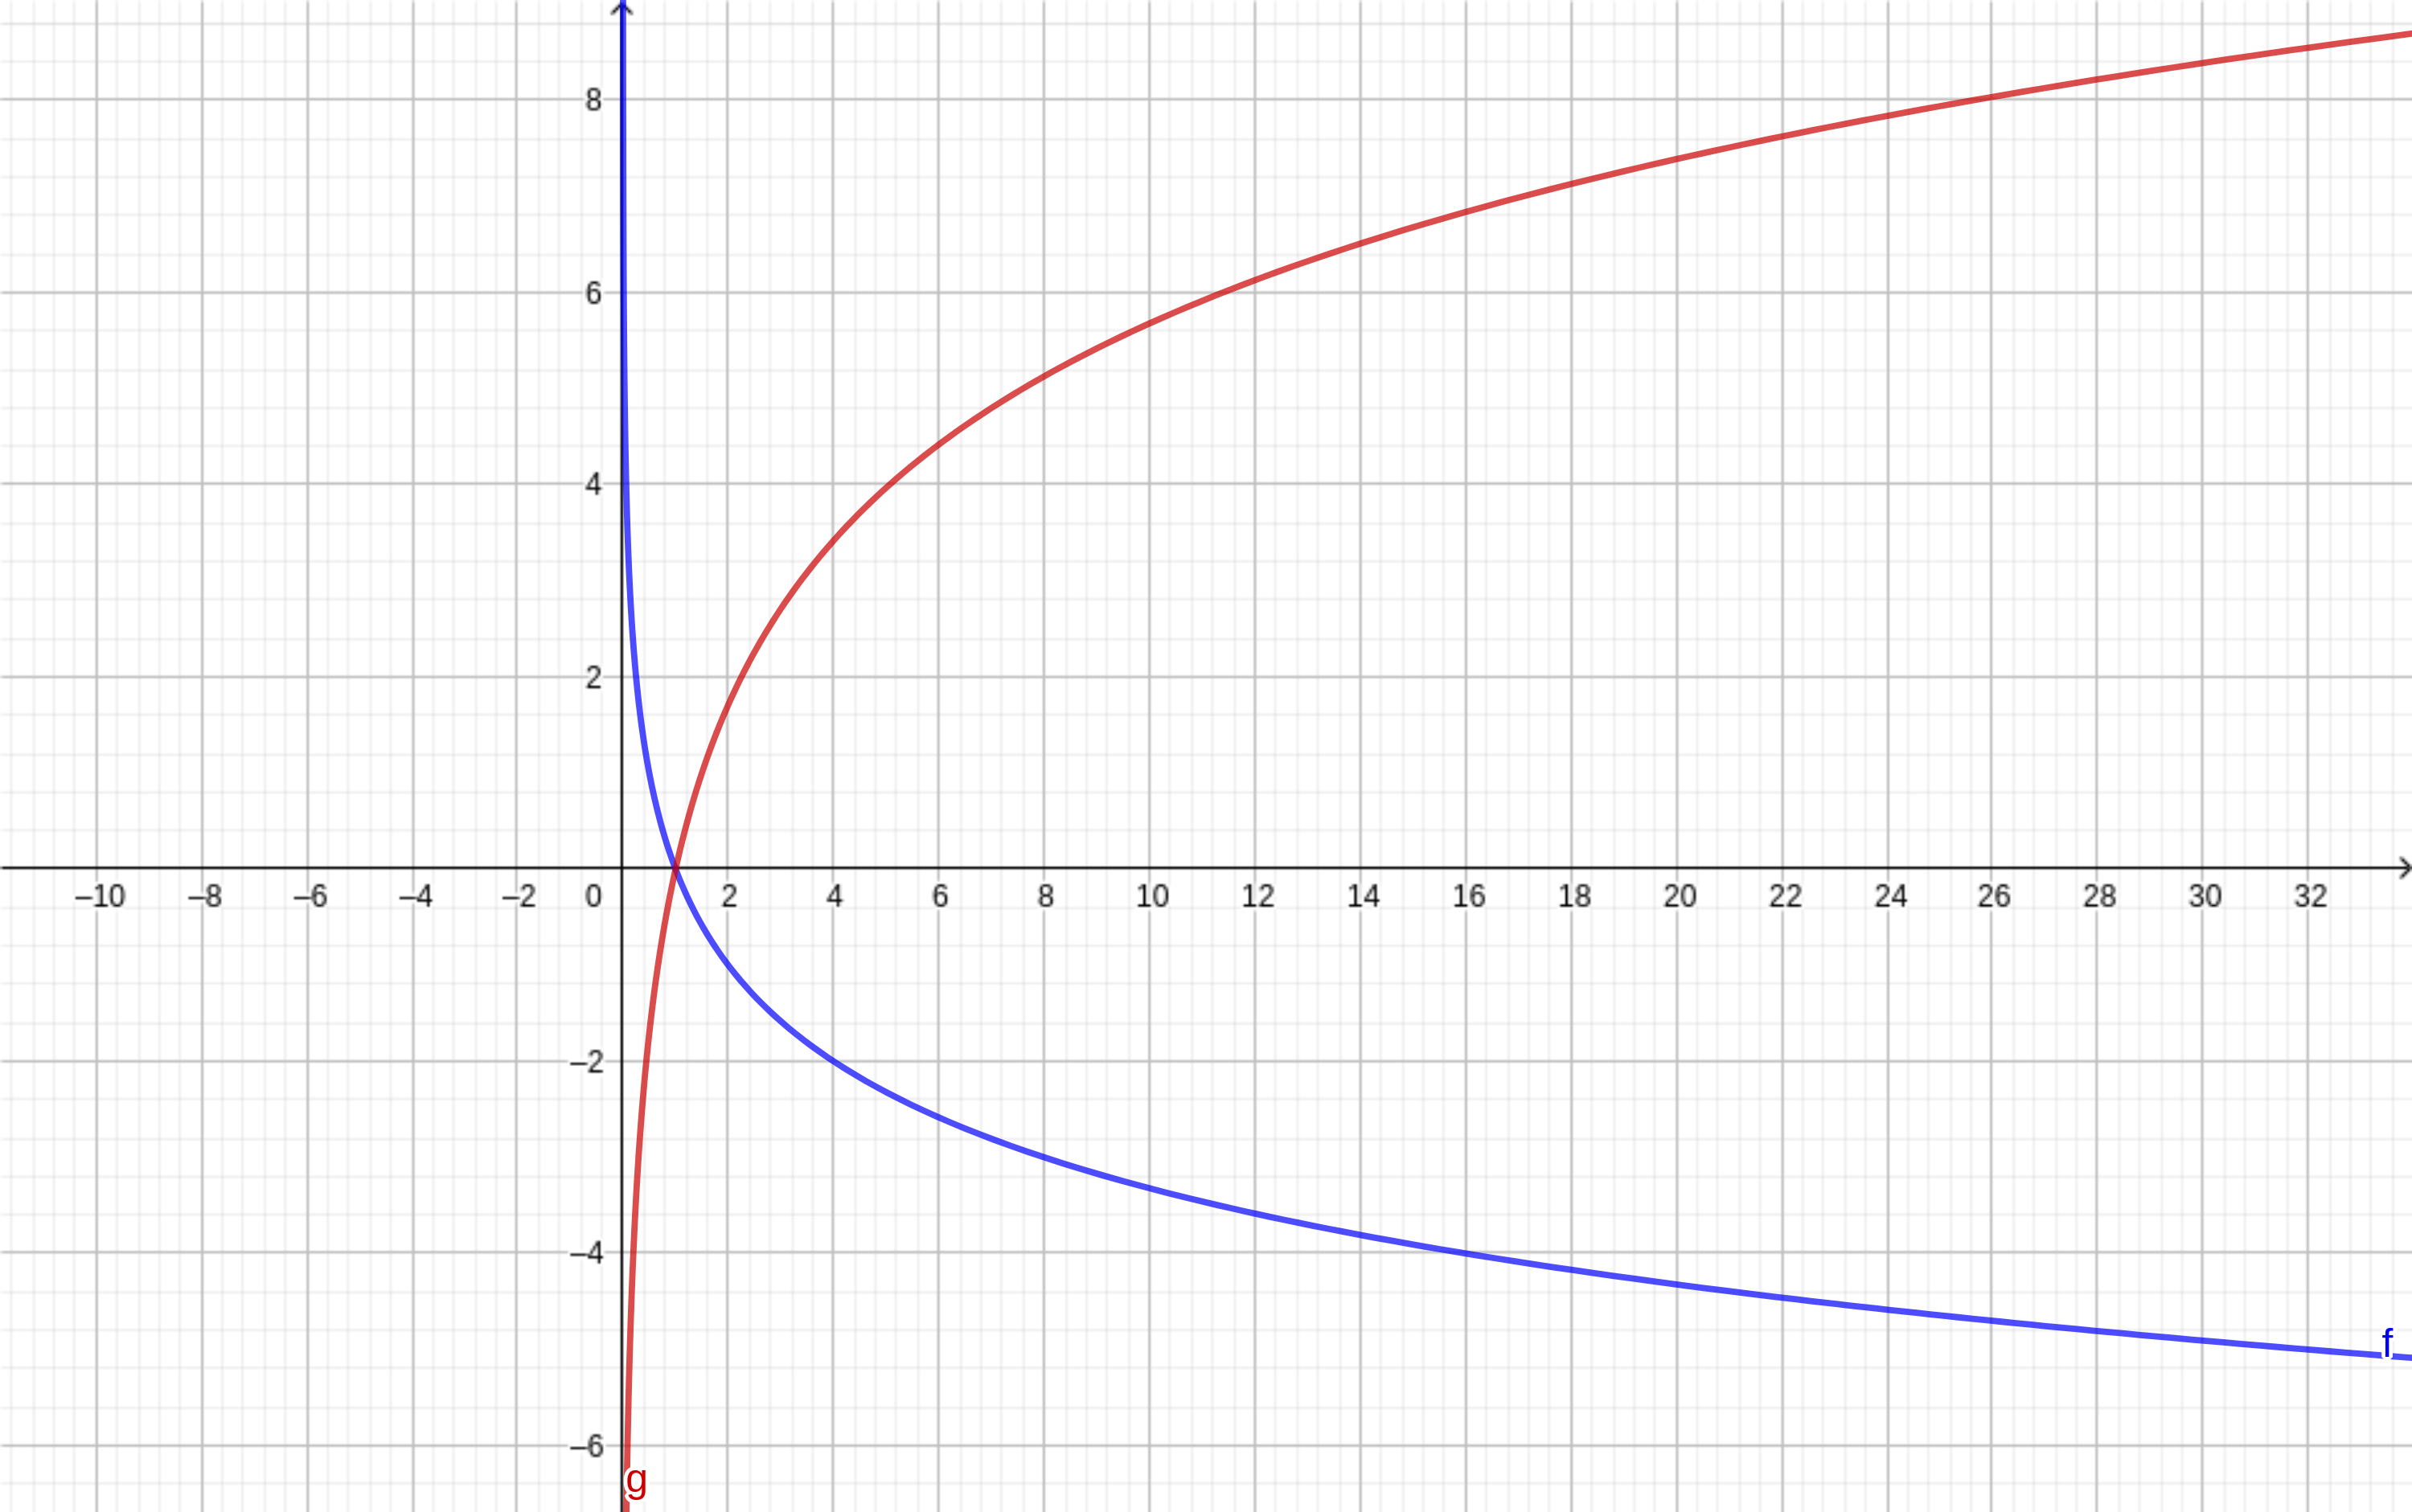
\includegraphics[width=0.5\linewidth]{imgs/log.png}
    \caption{Logaritmo: differenze tra base maggiore di 1 e compresa tra 0 e 1}
    \label{fig:log}
\end{figure}

\begin{itemize}
    \item Linea rossa ha base maggiore di 1
    \item Linea blue ha base compresa tra 0 e 1
\end{itemize}



\begin{figure}[h!]
    \centering
    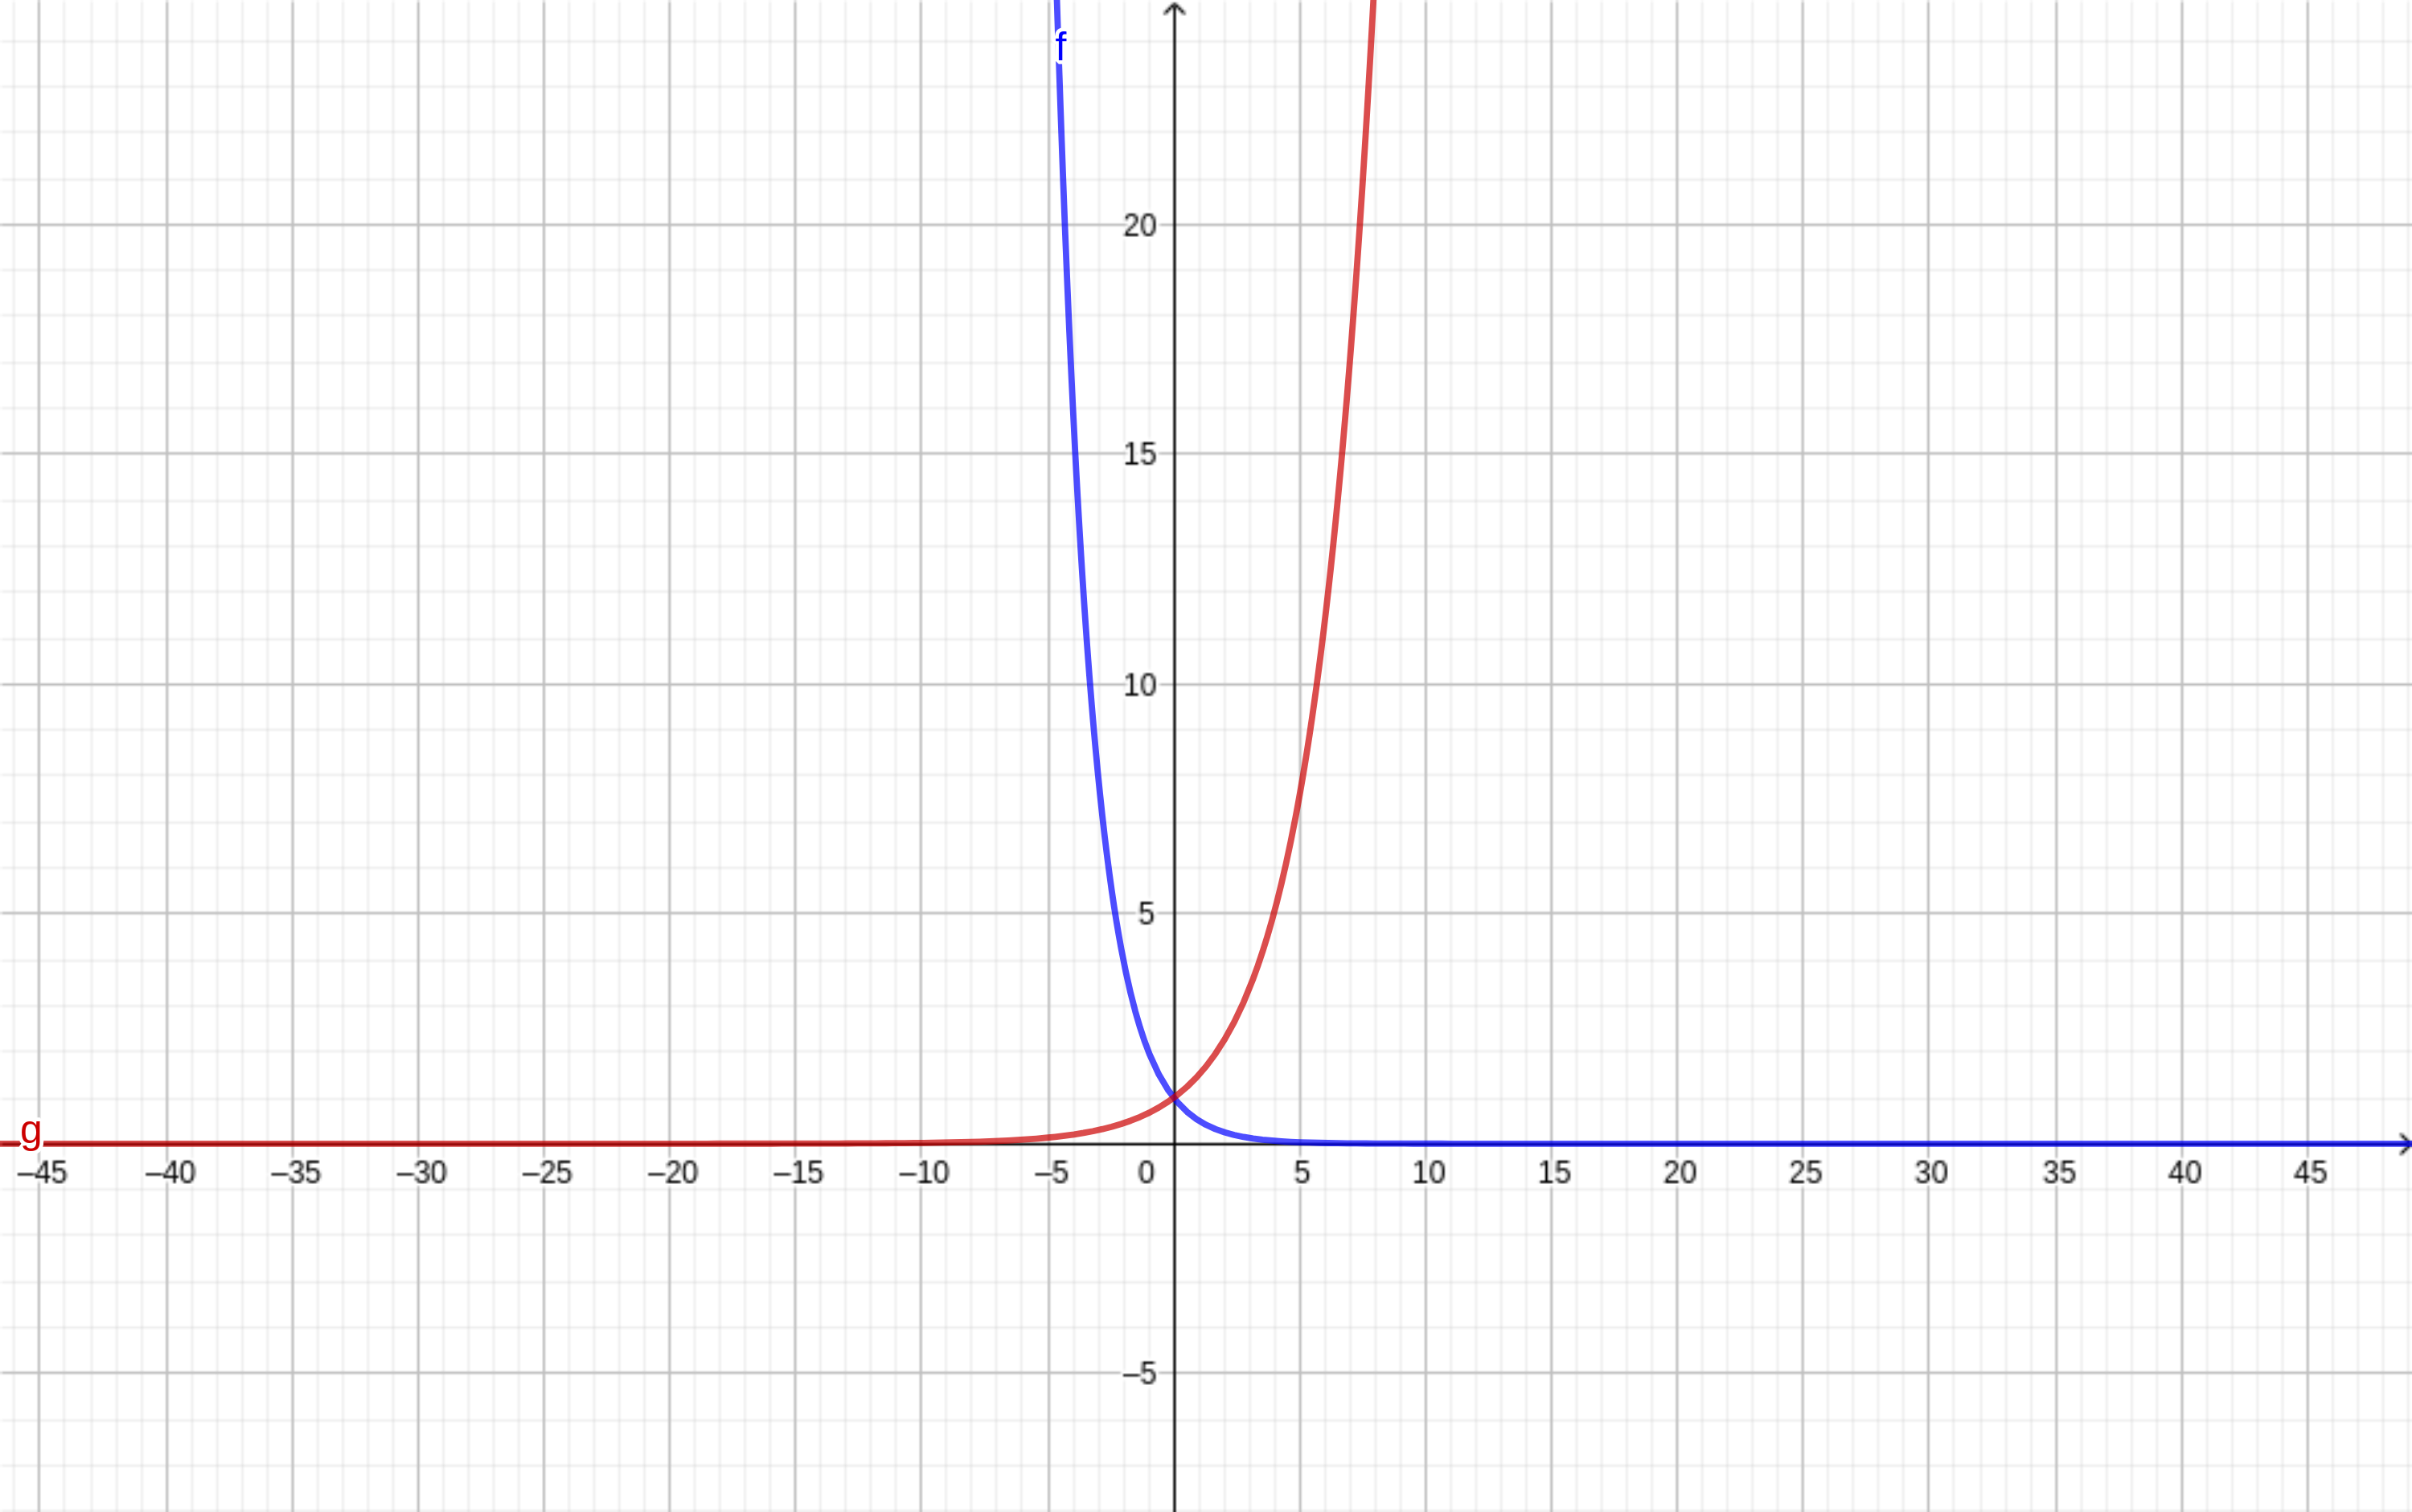
\includegraphics[width=0.5\linewidth]{imgs/exp.png}
    \caption{Esponenziale: differenze tra base maggiore di 1 e compresa tra 0 e 1}
    \label{fig:exp}
\end{figure}

\begin{itemize}
    \item Linea rossa ha base maggiore di 1
    \item Linea blue ha base compresa tra 0 e 1
\end{itemize}

\subsection{Funzioni trigonometriche}
Seno e coseno hanno dominio $D=[-1, 1]$, seno e dispari e coeno è pari.

\begin{equation*}
    \tan x = \frac{\sin x}{\cos x}
\end{equation*}

Il dominio è:
\begin{equation*}
    D(tan) = R \backslash \{ \frac{\pi}{2} + k\pi\}
\end{equation*}

\begin{equation*}
    \cot x = \frac{\cos x}{\sin x}
\end{equation*}

Il dominio è:
\begin{equation*}
    D(cot) = R \backslash \{ \pi + k\pi\}
\end{equation*}

Tan e cot sono dispari!!

\section{Estremo superiore/inferiore, minimo e massimo}

\subsection{Estremo superiore}
L'estremo superiore di un insieme $E \subseteq R$:

\textbf{Definizione}:


$E \subseteq X$ si dice limitato superiormente se $\exists M \in X \Leftrightarrow x\leq M, \forall x \in E$

\subsection{Estremo inferiore}
L'estremo inferiore di un insieme $E \subseteq R$:

\textbf{Definizione}:


$E \subseteq X$ si dice limitato inferiormente se $\exists m \in X \Leftrightarrow x\geq m, \forall x \in E$


Un'insieme si dice limitato quando è limitato superiormente e inferiormente.


\subsection{MAX}
\textbf{Definizione}:

Sia $E \subseteq X$, allora $X_M$ è il massimo per $E$ se:
\begin{equation*}
    \begin{cases}
        X_M \in E \\
        X_M \geq x, \forall x \in E
    \end{cases}
\end{equation*}

\subsection{MIN}
\textbf{Definizione}:

Sia $E \subseteq X$, allora $X_M$ è il minimo per $E$ se:
\begin{equation*}
    \begin{cases}
        X_m \in E \\
        X_m \leq x, \forall x \in E
    \end{cases}
\end{equation*}

\textbf{Osservazione}: se esiste un massimo l'insieme è limitato superiormente ecc.

\subsection{Maggiorante e minorante}

\textbf{Definizione}:
Sia $E \subseteq X$:

Un numero $k \in X$ si dice \textbf{maggiorante} se $k \geq x, \forall x \in E$.
$k$ non deve per forza far parte di $E$.



Un numero $k \in X$ si dice \textbf{minorante} se $k \leq x, \forall x \in E$.
$k$ non deve per forza far parte di $E$.



\textbf{Definizione}:

Chiameremo \textbf{Estremo inferiore} di $E$ $\inf(E)$(\textbf{il massimo dei minoranti}).


Chiameremo \textbf{Estremo superiore} di $E$ $\sup(E)$(\textbf{il minimo dei maggioranti}).


\section{Funzioni limite}

$f: D \subseteq R \rightarrow R$

\textbf{Definizione}:
$f$ si dice \textbf{limitata superiormente} se:
\begin{equation*}
    \exists M \in \Re \quad \Leftrightarrow \quad f(x) \leq M, \quad \forall x \in D
\end{equation*}

\textbf{Definizione}:
$f$ si dice \textbf{limitata inferiormente} se:
\begin{equation*}
    \exists m \in \Re \quad \Leftrightarrow \quad f(x) \geq m, \quad \forall x \in D
\end{equation*}

\textbf{Definizione}:
$f$ si dice \textbf{limitata} se lo è sia superiormente che inferiormente.

\section{Intorni e punti di accumulazione}

\textbf{Definizione}:
Un Intorno di $x_0 \in \Re$ è un'insieme della retta $\Re$ che contiene un'intervallo aperto del tipo:
\begin{equation*}
    I_\epsilon (x_0) = ] x_0 - \epsilon, \quad x_0 + \epsilon [
\end{equation*}

Con $\epsilon > 0$

\textbf{Definizione}:
Un'intorno di $+\infty$ è un'insieme $J \subseteq \Re$ che contiene intervalli aperti
del tipo $[M, \quad +\infty[$ con $M \in \Re$.

\textbf{Definizione}:
Sia $A \subseteq \Re$, e sia $X_0 \in \Re$, si dice che $x_0$ è \textbf{punto di accumulazione}
per $A$ se in ogni intorno di $J$ di $x_0$ esiste un punto $x$ diverso da $x_0$
che appartiene ad $A$.

\begin{equation*}
    \forall J \text{ di } x_0 \quad \exists x \neq x_0 \quad \Leftrightarrow x \in J \cap A
\end{equation*}

Sostanzialmente un punto di accumulazione(o p.d.a.) presenta dei punti attorno a se perchè si trova in un intervallo e non è un signolo punto.

\section{Limiti di funzioni}
\subsection{Teorema 1}
\textbf{Sono continue nel proprio dominio}:
\begin{enumerate}
    \item potenze
    \item funzioni trigonometriche
    \item logaritmo
\end{enumerate}
\subsection{Teorema 2}
Siano $f,g : I \rightarrow \Re, \quad X_0 \in I$

Supponendo che $f$ e $g$ siano continue in $x_0$, allora:
\begin{enumerate}
    \item $f \pm g$ è continua in $x_0$
    \item $f \cdot g$ è continua in $x_0$
    \item $\frac{f}{g}$ è continua in $x_0$, non in $g(x) =0$
\end{enumerate}

\subsection{Teorema colcolo dei limiti}

Siano:

\begin{equation*}
    \lim_{x \rightarrow x_0} f(x) = L \in \Re
\end{equation*}

\begin{equation*}
    \lim_{x \rightarrow x_0} g(x) = +\infty
\end{equation*}

allora:

\begin{enumerate}
    \item la somma risulta in più infinito
    \item la moltiplicazione dipende dal segno del limite finito
    \item la sottrazione f - g risulta in meno infinito 
\end{enumerate}

\section{Forme indefinite $[\frac{0}{0}]$}

\textbf{Esempio}:
\begin{equation}
    \lim_{x \rightarrow 0} \frac{x}{x^2 + 1}
\end{equation} 


    
\end{document}